\documentclass[runningheads]{llncs}

\usepackage{graphicx}
\usepackage{listings}
\usepackage{comment}


\begin{document}

% \thanks{Supported by organization x.}
\title{A Study in Cuda Usage}
\author{Pedro Carrega\inst{1} \and
Vasco Ferreira\inst{1}
}
%\authorrunning{F. Author et al.}

\institute{Departamento de Informática da Faculdade de Ciências da Universidade de Lisboa
\email{\{fc49080,fc49070\}@alunos.fc.ul.pt}}

\maketitle

\begin{abstract}
This paper was developed with the purpose to explain GPU programing and the improvements that can be made. To demonstrate this we used the Floyd-Warshall algorithm since it is very demanding for the CPU due to the high number of computations required. During our research we discovered that the available materials for learning GPGPU are quite difficult to understand for those who are looking to learn the basics of GPU programing. For that we developed this paper explaining from scratch GPGPU and some of the most significant improvements that can be made. We will start with a simple sequential solution of the algorithm in CUDA and from there go step by step till we use most of the tools and processing power that a GPU has to offer. This paper is helpful for someone who intends to learn the basics of GPGPU or could be used as a teaching guide in an IT course to introduce GPGPU to students.

\keywords{GPGPU  \and CUDA \and Floyd-Warshall.}
\end{abstract}
%
%
%
\section{Introduction}

The purpose of this paper is to teach GPU programing and the different improvements that can be made, showing the different improvements in each version so that the solution can perform even better taking advantage of the GPU optimizations. To demonstrate this, we used a well known problem that is the Floyd-Warshall algorithm. The algorithm calculates all the possible paths between two points and saves the shortest path. It was chosen because it requires a enormous amount of computation to get the final result since it is has O$(n^{3})$ complexity. With a high amount of entries, that is, a big matrix and so it can be very demanding for the CPU. This is where the GPU benefits due to its high number of threads.
\newline
For this paper all the examples will be in CUDA. %outras linguagens tem estas coisas?

To make a method to be computed in the GPU you need to declare it with the "\_\_global\_\_" \dots so that it will run on the GPU when called in the CPU. Each kernel runs a grid which is the group of blocks that are launched by the kernel, where each block is a set of threads. The grid can be represented as a one dimensional array, a two dimensional array or a three dimensional array. This can be used to improve the mapping of the work that each thread will do. 

When launching a kernel it has to be declared the number of threads per block and the number of blocks that are going to be used. It should be taken into consideration the fact that blocks are composed of warps which are a set of 32 threads, so when declaring the number of blocks being used, it should be a multiple of 32 since all threads in a warp use the same program counter. Therefor if the number of threads in the blocks is not multiple of 32 there will be threads that are busy, waiting for the other threads in their warp that are actually doing some work.

The composition of the kernel grid has a huge impact on performance, with that in mind a programmer of GPGPU should aim to use the largest amount of threads per block possible.

It also needs to be considered that the GPU does not have access to the memory used by the CPU, so all pointers used as input for the GPU kernel will have to be allocated and copied to the GPU global memory before being able to access it. The pointers of the memory that were allocated need to be passed through the parameters of the kernel call so that they can be used by the GPU. In case of a primitive type, it can be passed only by the parameters of the kernel (i.e. int) and does not need to allocate memory on the GPU memory manually(???????). After all the computations are finished, the result should be accessible by the CPU so that it can copy back the result to the CPU and do what it needs with it. To do that it needs to copy the result similarly to the opposite operation but this time from the device to the host. Then the memory that was allocated in the GPU memory should be freed so there are no memory leaks just like in the CPU. In the next figure you can see an example of a input being copied to the GPU, the call of the kernel, the corresponding composition of the grid which will be represented in the (NUMERO DA FIGURA COM A DISPOSICAO) and then the result being copied back to the CPU memory:
\newline

%need to put example code?
\begin{lstlisting}[language=C++, caption=CUDA Example]

//Consider the graph pointer a matrix of int with each entry 
with its corresponding value filled earlier and the same length on each axis
//graph_size being the size of each axis of the matrix
int* matrix_pointer_device;

cudaMalloc(&matrix_pointer_device, sizeof(int) * graph_size * graph_size);

//This will copy from the graph pointer to the matrix_pointer_device, that is copying the matrix in the CPU memory to the pointer with memory allocated in the GPU memory
cudaMemCpy(matrix_pointer_device, graph, sizeof(int) * graph_size * graph_size, cudaMemcpyHostToDevice);

//Definition of the parameters that describe the kernel grid

//Number of threads per blocks should be multiple of 32
dim3 threads(16,32);
//Number of blocks in the grid
dim3 blocks(4,2); 

//The number of total threads used by the kernel is equal to the total number of threads per block multiplied by the number of blocks used by the kernel.
//Launch of the kernel
computes<<<blocks, threads>>>(graph_size, matrix_pointer_device);

//Result being copied back to CPU memory
cudaMemCpy(graph, matrix_pointer_device, sizeof(int) * graph_size * graph_size, cudaMemcpyDeviceToHost);

//Freeing the GPU memory
cudaFree(cudaMemcpyDeviceToHost);

\end{lstlisting}



%e necessario aquele comentario final no codigo?



%Imagem que mostra a disposição da grid conforme os parametros passados para o kernel (nr de blocos e threads por bloco compondo o kernel)


\section{Background}

This is an optional section, as it depends on your project. In projects where a given specific knowledge is required to understand the article, you should give a brief introduction of the required concepts. In the case of genetic algorithms, you should present the basic algorithm in this section.


\section{Approach}

In this section, you should present your approach. Notice that an approach may be different than an implementation. An approach should be generic and ideally applied for different machines, virtual machines or languages. You should present algorithms or generic diagrams explaining the approach.

\section{Implementation Details}

In this section you can talk about details of how you implemented your approach. Depending on the detail of your approach, this might be an optional section.

As an example, I would detail how I implemented the phaser in the genetic algorithm, or how I implemented parallel mergesort on ForkJoin. Another aspect could be how to organize your arrays to minimize overhead in recursive calls.

\section{Versions}
\subsection{Sequential CPU}
In order to demonstrate the effectiveness of the usage of GPGPUs in the processing 
of some problems we started by implementing our problem in the CPU so we could use the results as a reference point to our others solutions.
%nao sei se devia por este paragrafo abaixo

This solution will only use one thread of the CPU as the purpose of this paper is to demonstrate the impact of the improvements that can be made on the GPGPU.
The graph we will be using for the Floyd-Warshall problem will be a two dimensional graph, in another words, a 2D grid.
With that in mind, we by creating 3 \textit{for} cycles each will start at 0 and will iterate a number of times corresponding to the size of the graph.
The second and third cycle will correspond to the X and Y coordinates, respectively, 
while the first cycle will match an intermediate point for which the shortest path will be computed.
%nao sei se meto esta ultima parte.
Inside the last cycle it will be compared the direct distance of X to Y with the addition of the distances 
of X to K and K to Y, in case the latter is smaller the distance of X to Y is updated with the value of the addition.

\subsection{Sequential GPU}
To start our learning of how to program in the GPU we will start by doing the most basic implementation possible, 
one thread computing the entirety of the Floyd-Warshall problem.
GPU functions work like any other CPU functions barring two simple differences. 

First, a GPU function has either the \textit{\_\_global\_\_} or the \textit{\_\_device\_\_} \dots%k usar aqui? tag? keyword?
where \textit{\_\_global\_\_} is a function that will be called by the CPU but run on the GPU 
and \textit{\_\_device\_\_} is a function that is called by the GPU to be run by the GPU. 
This \dots can also be used to initialize a global variable on the GPU.

Second, the syntax of the call of a GPU function also differs. Kernels work on a grid basis, and such, you need to indicate the grid your program will be working on. 
That indication is made by placing
\begin{math} <<< X, Y >>> \end{math}
after the name of the function, where X represents the number of blocks to be used and Y the number of threads to be used per block, respectively. 

Having copied our graph to the GPU memory, we call our kernel with one block and one thread per block, 
Inside our GPU function we apply the same programing logic that was applied for the sequential CPU version of the Floyd-Warshall problem. 
We create 3 \textit{for} cycles to iterate through our graph and compute our problem.


\subsection{Parallel GPU}
Using a single thread to compute a problem on the GPU goes against it's strengths. 
Due to the low core clock speed, the strength of the GPU comes from it's high thread count being able to compute multiple values at the same time. 

When running a function parallel on the GPU each thread will run it's own instance of that same function, 
in other words, the implementation of the function now needs to take into consideration how we partition the work load for each thread. 
Having decided the number of threads per blocks we want to use, the most common way to split the work load is to 
use that number to divide the size of our problem, this way obtaining the number of blocks we are going to use to compute our problem. 

Obviously we are going to follow that same logic, but seeing that our problem uses a 2D grid, 
applying a 2D grid to our blocks and threads. Such can be made using \textit{dim3()} \dots, 
and so our kernel call will look like: \newline\small{\textit{parallelGPU}
\begin{math} <<< \end{math}
\textit{dim3(GRAPH\_SIZE/NThreads,GRAPH\_SIZE/NThreads),\newline dim3(NThreads,NThreads)}
\begin{math} >>> \end{math}}. \newline
Where GRAPH\_Size is the size of our graph and NThreads the number of threads we decided to use.

Regarding the implementation of our function, we have to change it completely.
The kernel is now called K times by the CPU, where K goes from 0 to GRAPH\_SIZE, 
each thread will now be attributed two coordinates determined by their coordinates in the 2D grid. 
If the coordinates are withing the scope of the problem they will try to compute the shortest path between X to Y, using the value of K provided by the CPU when the kernel is called, updating the value if needed. 
%In order to improve performance, to the values of X and Y are added the block dimension multiplied by the dimension of the grid. After, if the coordinates are still within the scope of the problem, the thread will compute again using the new coordinates.%compute? 

\subsection{Work Load}

How we partition the work load for each thread may have a big impact on the performance of our solution. Like mentioned before, the major strength of the GPU is it's high thread count so that it can compute multiple values at the same time.
During our research into the topic we came up with the following guidelines in order to optimize work load: %algo me melhor k "came up with"
\begin{enumerate}
	\item Every thread works the same amount
	\item Use the most amount of threads possible
	\item Avoid using the scheduler
	\newline
\end{enumerate}
%nao gosto deste paragrafo
1. Considering every thread follows the program counter of the warp, meaning the thread is only allowed to compute a certain line when the warp allows it.
Threads with less work load might find themselves in a situation where they must sit idle waiting for others threads to catch up.
This scenario is avoided by a correct split of the work load, making every thread in the same warp be synchronized on the computation it needs to execute.
\newline
\newline
%e deste
2. Simply put, the more threads you have available to compute your problem the more you can divide your problem. A major cavite however is to not use more threads than those that are available on the GPU. When the number of threads used is bigger than those available the GPU scheduler begins to be involved a major overhead is added to the computation cutting a lot of the performance offered by the GPU.
\newline
\newline
%ja disse k nao tou inspirado hj?
3. Like mentioned before, using the GPU scheduler adds a major overhead to the computation, so it makes sense that we try to avoid using it.
One possible workaround, on a kernel call that uses loops and the problem is bigger than the number of threads offered by the GPU, is to increment the value of the coordinates variable by the product of the dimension of the block by the dimension of the grid. Doing this will allows us to reuse certain threads without having to rely on the GPU scheduler.
\newline
\newline
To show the importance of using a correct work load we will implement another solution to the Floyd-Warshall problem. First we need to decide how many blocks and threads we will be using, being both in a 2D grid. For the threads you should use the number that makes most sense considering your system, in our case that number is 8. Regarding the number of blocks we decided to use the squared root of the number of blocks allowed per multiprocessor times the number of multiprocessors present on our GPU. We then determined how much positions each thread would need to compute and send that value with our kernel call.

We determine the coordinates like previous implementations with the difference that to that number we multiply the number of positions each thread will need to compute. %fazemos isso pk....
Then we create two \textit{for} cycles that go from those coordinates to that number plus the number of positions the thread will need to compute. If the coordinates are within the scope of the problem the thread will then compute.

\subsection{Synchronization}

CUDA offers it's users some forms of synchronization, allowing it's users to have a barrier on theirs implementations.
The most common forms of synchronization is using \_\_syncthreads(), which blocks the thread till all threads within the same block call it, and using Atomic variables. Atomic variables have the benefit of offering GPU wide synchronization but usage of such variables is very slow, making them only useful on certain scenarios.

Considering the Floyd-Warshall only has one barrier point, we can use synchronization to reduce the number of kernel calls to just one.
We will be using the same implementation used on the previous iteration of our solution, but slightly modifying it so it uses synchronization.
We'll start by defining a global variable called \textit{barrier} on the GPU so that we can have GPU wide synchronization, this variable will start at 0. 
Being a variable whose propose is synchronization, all operations on it will be atomic. 
But like mentioned before atomic operations carry an heavy performance cost, so to reduce the usage only one thread per block will be computing atomic operations on the variable.
Since now we will only be calling the kernel once every thread must now store it's own variable K, which will be iterated by 1 every computing cycle. 
At the end of the computing cycle one thread per block will increment the value of barrier by one and then be stuck in a empty loop while it waits for every block to increment by 1 the value of barrier. 
We will be using \_\_syncthreads() so that the other threads await for the synchronization between blocks.


\subsection{Shared Memory}
Shared memory is a type of memory located on-chip, meaning it is much faster then global memory. In fact shared memory latency is roughly 
100x lower than uncached global memory latency (provided that there are no bank conflicts between the threads). It is allocated per 
thread block, so all threads in the block have access to the same shared memory. The size of memory that can be used is limited, it depends on the GPU
used, so when using it be aware of the GPU limitations.
Each thread has a local storage which is on-chip as the shared memory, but it is even faster due to being implemented as registers with spill over
into L1 cache. This type of memory should be used every time it is possible, as the shared memory it is limited but even more.

Considering that, it should always be taken into advantage the usage of both registry and shared memory. The registry variables are created when defining
new variables inside of the kernel implementation, the shared memory are the variables that are declared also inside of the kernel but with \_\_shared\_\_.

The following implementation follows the logic explained in a previous subsection, but now using shared memory to save entries that will be used 
multiple times, this way we avoid multiple reads from the global memory saving some time in each thread execution resulting in a better performance of the GPU kernel.

MOSTRAR IMPLEMENTACAO DO KERNEL QUE FIZEMOS

The logic in this implementation is that when iterating though a small part the matrix, some positions are being read multiple times, in this specific 
example lets consider workPerThread with the value 10, in this case each iteration of the outside loop will iterate over the Y axis the 10 times, when 
doing so the D(x,k) will not change, so by writing this value in the corresponding entry of the matrix in the shared memory we save some time. The logic 
in writing the D(k,y) is almost the same, when doing the first iteration of the outside loop, we will be reading from global memory all the possible 
values of D(k,y) for that thread, by doing so it has an unnecessary overhead. To prevent that, we will have a shared three dimensional array, where the 
first two dimensions represent the thread position in the block, were each thread of the block will have each position and the third dimension will be 
the different D(k,y) entries for that thread. Note that it should only be done in the first iteration of the outside loop as explained before. 
In this case it needs to be three dimensional array since it is the inside loop, were in the D(x,k) improvement, we only need one position of the matrix 
for each thread because that value will be updated at the beginning of each iteration of the outside loop.

\section{Evaluation}

\subsection{Experimental Setup}

%To be decided

\subsection{Results}

To show the results and effectiveness of our solutions we ran two sets of tests:
\begin{itemize}
	\item We ran both sequential versions with the graph size at 2000, in order to show the weakness of the GPU in single threaded tasks. \item We ran all our implementations, minus the sequential GPU, in order to show the impact of our improvements made on the computation of our problem.
\end{itemize}

\begin{comment}
	

In this section you should present the results. Do not forget to explain where the data came from. 

You should include (ideally vectorial) plots, with a descriptive caption. Make sure all the plots (Like Figure~\ref{fig1} are well identified and axis and metrics are defined.

\begin{figure}[htbp]
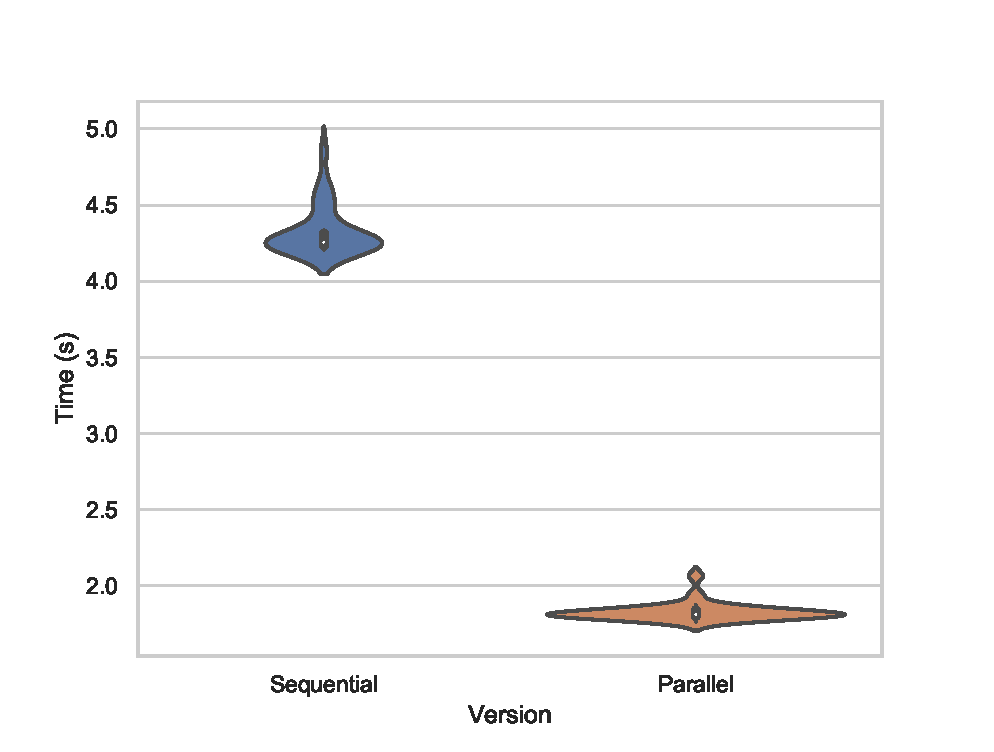
\includegraphics[width=\textwidth]{code/performance.eps}
\caption{Comparison of the performance of sequential and parallel versions of the algorithm.} \label{fig1}
\end{figure}
\end{comment}

\subsection{Discussion}



\begin{comment}
Here you should discuss the results on a high level. For instance, based on our results, the parallelization of the merge-sort is relevant as no other parallel work occurs at the same time, and the complexity $O(N log(N))$ can have a large impact when the number of individuals is high.
\end{comment}

\section{Related Work}

This section can be either the second one, or the second-to-last. In the case where knowledge of other competing works is required, it could come before. But if you are confident on what you did, it should appear at the end, where you can compare existing works against yours. An example is below:

Chu and Beasley proposed a Genetic Algorithm for the Multidimensional Knapsack Problem \cite{DBLP:journals/heuristics/ChuB98}. This work introduces a heuristic as a repair operator. Our work makes no optimization with regards to the problem domain, making it more generic and supporting other problems.


When using BibTeX references, I suggest using DBLP\footnote{\url{https://dblp.org}}, leaving Google Scholar as a backup, since DBLP has more correct and detailed information about research papers.

\section{Conclusions}

Here you should resume the major conclusions taken from discussion. Ideally, these should align with the objectives introduced in the introduction.


You should also list the future work, i. e., tasks and challenges that were outside your scope, but are relevant.

\section*{Acknowledgements}

First Author wrote the part of the program implemented the phasers. Second Author implemented the MergeSort in parallel. 

Both authors wrote this paper, with First Author focusing on the introduction, related work and conclusions while the Second Author focused on approach and evaluation.

Each author spent around 30 hours on this project.

\bibliographystyle{splncs04}
\bibliography{bibliography}

\end{document}
